%!TEX root = main.tex
%
\begin{assumptions}
     According to COVID-19 dynamics \Cref{eqn:base_dynamics}, we
     made the following modeling hypotheses about the regarding vaccine.
     \begin{enumerate}[label={\textbf{(VH-\arabic*)}}]
        \item
            Vaccine is preventive and only reduce susceptibility.
            
        \item
            The vaccination camping omits testing to detect seroprevalence.
            Thus Exposed, Infected Asymptomatic and Recovered Asymptomatic
            individuals are undetected but would obtain a vaccine dose
            \textemdash which in this model represents a waste of resources
        \item
            Individuals under lockdown are also vaccinated
        \item
            The vaccine is leaky and with efficacy $\epsilon \in[0.7, .975]$
        \item   
            Vaccine induced immunity last \SI{2}{years}
        \item   
            Natural immunity last a period of \SI{180}{days} 
     \end{enumerate}
\end{assumptions}
\begin{figure*}[tbh]
    \centering
      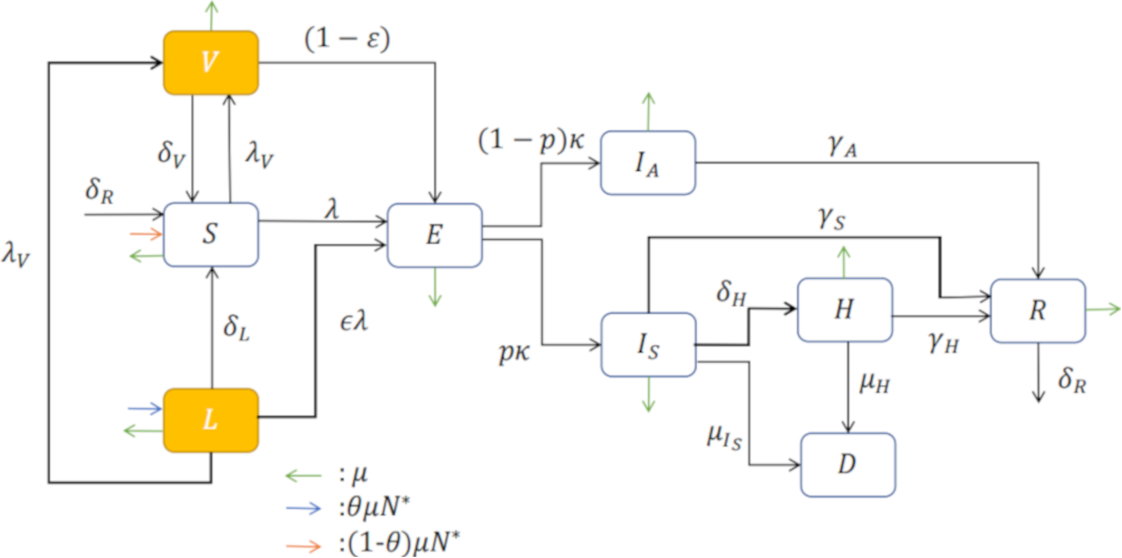
\includegraphics[scale=0.7, keepaspectratio]{Diagram_Vaccination.pdf}
    %

\tikzset{every picture/.style={line width=0.75pt}} %set default line width to 0.75pt        

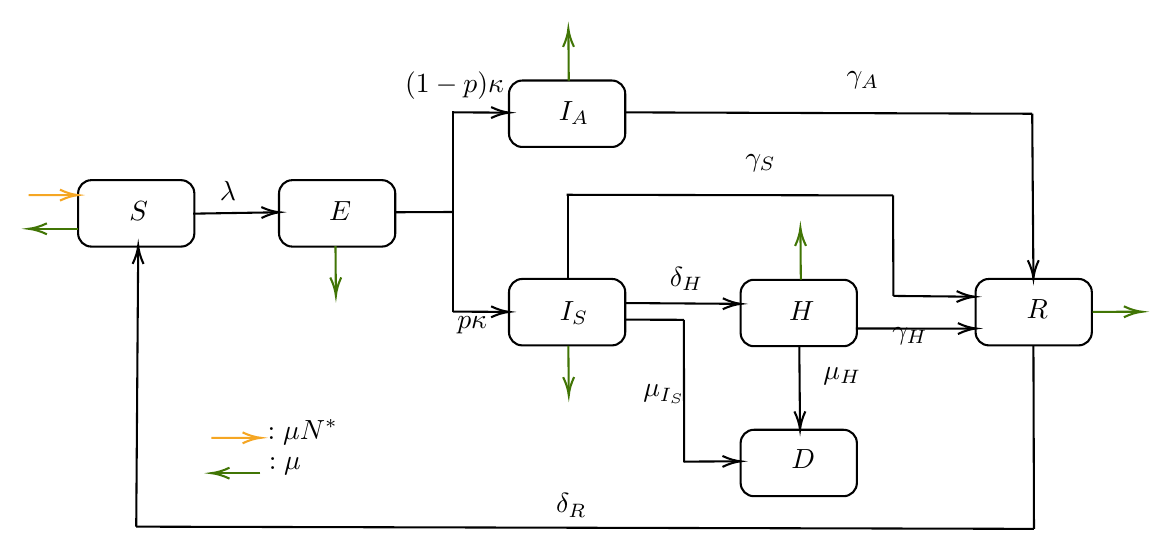
\begin{tikzpicture}[x=0.75pt,y=0.75pt,yscale=-0.8,xscale=0.8]
%uncomment if require: \path (0,391); %set diagram left start at 0, and has height of 391

%Rounded Rect [id:dp9338258576556762] 
\draw   (40,138) .. controls (40,133.58) and (43.58,130) .. (48,130) -- (102,130) .. controls (106.42,130) and (110,133.58) .. (110,138) -- (110,162) .. controls (110,166.42) and (106.42,170) .. (102,170) -- (48,170) .. controls (43.58,170) and (40,166.42) .. (40,162) -- cycle ;
%Rounded Rect [id:dp03550846434827437] 
\draw   (161,138) .. controls (161,133.58) and (164.58,130) .. (169,130) -- (223,130) .. controls (227.42,130) and (231,133.58) .. (231,138) -- (231,162) .. controls (231,166.42) and (227.42,170) .. (223,170) -- (169,170) .. controls (164.58,170) and (161,166.42) .. (161,162) -- cycle ;
%Rounded Rect [id:dp2096597210016533] 
\draw   (299.5,78) .. controls (299.5,73.58) and (303.08,70) .. (307.5,70) -- (361.5,70) .. controls (365.92,70) and (369.5,73.58) .. (369.5,78) -- (369.5,102) .. controls (369.5,106.42) and (365.92,110) .. (361.5,110) -- (307.5,110) .. controls (303.08,110) and (299.5,106.42) .. (299.5,102) -- cycle ;
%Rounded Rect [id:dp4192775592826552] 
\draw   (299.5,197.5) .. controls (299.5,193.08) and (303.08,189.5) .. (307.5,189.5) -- (361.5,189.5) .. controls (365.92,189.5) and (369.5,193.08) .. (369.5,197.5) -- (369.5,221.5) .. controls (369.5,225.92) and (365.92,229.5) .. (361.5,229.5) -- (307.5,229.5) .. controls (303.08,229.5) and (299.5,225.92) .. (299.5,221.5) -- cycle ;
%Rounded Rect [id:dp9412674774350195] 
\draw   (580.5,197.5) .. controls (580.5,193.08) and (584.08,189.5) .. (588.5,189.5) -- (642.5,189.5) .. controls (646.92,189.5) and (650.5,193.08) .. (650.5,197.5) -- (650.5,221.5) .. controls (650.5,225.92) and (646.92,229.5) .. (642.5,229.5) -- (588.5,229.5) .. controls (584.08,229.5) and (580.5,225.92) .. (580.5,221.5) -- cycle ;
%Rounded Rect [id:dp7750331540351684] 
\draw   (439,288.33) .. controls (439,283.92) and (442.58,280.33) .. (447,280.33) -- (501,280.33) .. controls (505.42,280.33) and (509,283.92) .. (509,288.33) -- (509,312.33) .. controls (509,316.75) and (505.42,320.33) .. (501,320.33) -- (447,320.33) .. controls (442.58,320.33) and (439,316.75) .. (439,312.33) -- cycle ;
%Rounded Rect [id:dp22729858034129236] 
\draw   (439,198) .. controls (439,193.58) and (442.58,190) .. (447,190) -- (501,190) .. controls (505.42,190) and (509,193.58) .. (509,198) -- (509,222) .. controls (509,226.42) and (505.42,230) .. (501,230) -- (447,230) .. controls (442.58,230) and (439,226.42) .. (439,222) -- cycle ;
%Straight Lines [id:da8056305543799926] 
\draw    (109.33,150.17) -- (159.33,149.37) ;
\draw [shift={(161.33,149.33)}, rotate = 539.0799999999999] [color={rgb, 255:red, 0; green, 0; blue, 0 }  ][line width=0.75]    (10.93,-3.29) .. controls (6.95,-1.4) and (3.31,-0.3) .. (0,0) .. controls (3.31,0.3) and (6.95,1.4) .. (10.93,3.29)   ;
%Straight Lines [id:da2787683579538649] 
\draw    (230.78,149.33) -- (265.67,149.17) ;
%Straight Lines [id:da21916666537860907] 
\draw    (265.67,89.17) -- (297.67,89.32) ;
\draw [shift={(299.67,89.33)}, rotate = 180.28] [color={rgb, 255:red, 0; green, 0; blue, 0 }  ][line width=0.75]    (10.93,-3.29) .. controls (6.95,-1.4) and (3.31,-0.3) .. (0,0) .. controls (3.31,0.3) and (6.95,1.4) .. (10.93,3.29)   ;
%Straight Lines [id:da8438200798129222] 
\draw    (265.67,88.6) -- (265.67,209.17) ;
%Straight Lines [id:da7337155371803761] 
\draw    (265.67,209.17) -- (297.67,209.32) ;
\draw [shift={(299.67,209.33)}, rotate = 180.28] [color={rgb, 255:red, 0; green, 0; blue, 0 }  ][line width=0.75]    (10.93,-3.29) .. controls (6.95,-1.4) and (3.31,-0.3) .. (0,0) .. controls (3.31,0.3) and (6.95,1.4) .. (10.93,3.29)   ;
%Straight Lines [id:da509274682669141] 
\draw    (369.43,204) -- (424.2,204.39) -- (437.2,204.49) ;
\draw [shift={(439.2,204.5)}, rotate = 180.41] [color={rgb, 255:red, 0; green, 0; blue, 0 }  ][line width=0.75]    (10.93,-3.29) .. controls (6.95,-1.4) and (3.31,-0.3) .. (0,0) .. controls (3.31,0.3) and (6.95,1.4) .. (10.93,3.29)   ;
%Straight Lines [id:da3183759306298827] 
\draw    (405,299.5) -- (437,299.34) ;
\draw [shift={(439,299.33)}, rotate = 539.72] [color={rgb, 255:red, 0; green, 0; blue, 0 }  ][line width=0.75]    (10.93,-3.29) .. controls (6.95,-1.4) and (3.31,-0.3) .. (0,0) .. controls (3.31,0.3) and (6.95,1.4) .. (10.93,3.29)   ;
%Straight Lines [id:da6861028849351065] 
\draw    (370,214) -- (404.8,214.1) ;
%Straight Lines [id:da9190171216881116] 
\draw    (404.8,214.1) -- (405,300) ;
%Straight Lines [id:da03313994658252273] 
\draw    (508.33,219.33) -- (565.2,219.39) -- (578.78,219.34) ;
\draw [shift={(580.78,219.33)}, rotate = 539.78] [color={rgb, 255:red, 0; green, 0; blue, 0 }  ][line width=0.75]    (10.93,-3.29) .. controls (6.95,-1.4) and (3.31,-0.3) .. (0,0) .. controls (3.31,0.3) and (6.95,1.4) .. (10.93,3.29)   ;
%Straight Lines [id:da6934604539767528] 
\draw    (474.33,230) -- (474.76,278.22) ;
\draw [shift={(474.78,280.22)}, rotate = 269.49] [color={rgb, 255:red, 0; green, 0; blue, 0 }  ][line width=0.75]    (10.93,-3.29) .. controls (6.95,-1.4) and (3.31,-0.3) .. (0,0) .. controls (3.31,0.3) and (6.95,1.4) .. (10.93,3.29)   ;
%Straight Lines [id:da6916456040068684] 
\draw    (369,89.17) -- (614.6,90) ;
%Straight Lines [id:da7246498566982733] 
\draw    (614.6,90) -- (615.32,187.17) ;
\draw [shift={(615.33,189.17)}, rotate = 269.58] [color={rgb, 255:red, 0; green, 0; blue, 0 }  ][line width=0.75]    (10.93,-3.29) .. controls (6.95,-1.4) and (3.31,-0.3) .. (0,0) .. controls (3.31,0.3) and (6.95,1.4) .. (10.93,3.29)   ;
%Straight Lines [id:da5396778112959429] 
\draw    (335,139.17) -- (335,189.5) ;
%Straight Lines [id:da7180507787496266] 
\draw    (334.2,138.8) -- (530.8,139.2) ;
%Straight Lines [id:da3365589163505732] 
\draw    (531,199.71) -- (578,200.18) ;
\draw [shift={(580,200.2)}, rotate = 180.57] [color={rgb, 255:red, 0; green, 0; blue, 0 }  ][line width=0.75]    (10.93,-3.29) .. controls (6.95,-1.4) and (3.31,-0.3) .. (0,0) .. controls (3.31,0.3) and (6.95,1.4) .. (10.93,3.29)   ;
%Straight Lines [id:da7818385183529692] 
\draw    (530.8,139.2) -- (531,199.71) ;
%Straight Lines [id:da7484740849372823] 
\draw    (75,338.67) -- (76.19,171.5) ;
\draw [shift={(76.2,169.5)}, rotate = 450.41] [color={rgb, 255:red, 0; green, 0; blue, 0 }  ][line width=0.75]    (10.93,-3.29) .. controls (6.95,-1.4) and (3.31,-0.3) .. (0,0) .. controls (3.31,0.3) and (6.95,1.4) .. (10.93,3.29)   ;
%Straight Lines [id:da29835177923282885] 
\draw    (75,338.67) -- (615.67,340) ;
%Straight Lines [id:da7139155616312535] 
\draw    (615.33,229.67) -- (615.67,340) ;
%Straight Lines [id:da20994732667721105] 
\draw [color={rgb, 255:red, 245; green, 166; blue, 35 }  ,draw opacity=1 ][fill={rgb, 255:red, 65; green, 117; blue, 5 }  ,fill opacity=1 ]   (10.25,139.04) -- (38,139) ;
\draw [shift={(40,139)}, rotate = 539.9200000000001] [color={rgb, 255:red, 245; green, 166; blue, 35 }  ,draw opacity=1 ][line width=0.75]    (10.93,-3.29) .. controls (6.95,-1.4) and (3.31,-0.3) .. (0,0) .. controls (3.31,0.3) and (6.95,1.4) .. (10.93,3.29)   ;
%Straight Lines [id:da9409632697808414] 
\draw [color={rgb, 255:red, 65; green, 117; blue, 5 }  ,draw opacity=1 ]   (39.75,159.29) -- (12.25,159.29) ;
\draw [shift={(10.25,159.29)}, rotate = 360] [color={rgb, 255:red, 65; green, 117; blue, 5 }  ,draw opacity=1 ][line width=0.75]    (10.93,-3.29) .. controls (6.95,-1.4) and (3.31,-0.3) .. (0,0) .. controls (3.31,0.3) and (6.95,1.4) .. (10.93,3.29)   ;
%Straight Lines [id:da671739616587531] 
\draw [color={rgb, 255:red, 65; green, 117; blue, 5 }  ,draw opacity=1 ]   (195,169.79) -- (195.23,197.54) ;
\draw [shift={(195.25,199.54)}, rotate = 269.52] [color={rgb, 255:red, 65; green, 117; blue, 5 }  ,draw opacity=1 ][line width=0.75]    (10.93,-3.29) .. controls (6.95,-1.4) and (3.31,-0.3) .. (0,0) .. controls (3.31,0.3) and (6.95,1.4) .. (10.93,3.29)   ;
%Straight Lines [id:da4612478738976049] 
\draw [color={rgb, 255:red, 65; green, 117; blue, 5 }  ,draw opacity=1 ]   (335.25,229.79) -- (335.48,257.54) ;
\draw [shift={(335.5,259.54)}, rotate = 269.52] [color={rgb, 255:red, 65; green, 117; blue, 5 }  ,draw opacity=1 ][line width=0.75]    (10.93,-3.29) .. controls (6.95,-1.4) and (3.31,-0.3) .. (0,0) .. controls (3.31,0.3) and (6.95,1.4) .. (10.93,3.29)   ;
%Straight Lines [id:da6463966696699537] 
\draw [color={rgb, 255:red, 65; green, 117; blue, 5 }  ,draw opacity=1 ]   (335.5,70.04) -- (335.27,40.79) ;
\draw [shift={(335.25,38.79)}, rotate = 449.54] [color={rgb, 255:red, 65; green, 117; blue, 5 }  ,draw opacity=1 ][line width=0.75]    (10.93,-3.29) .. controls (6.95,-1.4) and (3.31,-0.3) .. (0,0) .. controls (3.31,0.3) and (6.95,1.4) .. (10.93,3.29)   ;
%Straight Lines [id:da5390055225547872] 
\draw [color={rgb, 255:red, 65; green, 117; blue, 5 }  ,draw opacity=1 ]   (475.25,189.92) -- (475.02,160.67) ;
\draw [shift={(475,158.67)}, rotate = 449.54] [color={rgb, 255:red, 65; green, 117; blue, 5 }  ,draw opacity=1 ][line width=0.75]    (10.93,-3.29) .. controls (6.95,-1.4) and (3.31,-0.3) .. (0,0) .. controls (3.31,0.3) and (6.95,1.4) .. (10.93,3.29)   ;
%Straight Lines [id:da5965287355289506] 
\draw [color={rgb, 255:red, 65; green, 117; blue, 5 }  ,draw opacity=1 ]   (651,209.29) -- (678.75,209.25) ;
\draw [shift={(680.75,209.25)}, rotate = 539.9200000000001] [color={rgb, 255:red, 65; green, 117; blue, 5 }  ,draw opacity=1 ][line width=0.75]    (10.93,-3.29) .. controls (6.95,-1.4) and (3.31,-0.3) .. (0,0) .. controls (3.31,0.3) and (6.95,1.4) .. (10.93,3.29)   ;
%Straight Lines [id:da8186275398290976] 
\draw [color={rgb, 255:red, 245; green, 166; blue, 35 }  ,draw opacity=1 ]   (120.25,285.21) -- (148,285.17) ;
\draw [shift={(150,285.17)}, rotate = 539.9200000000001] [color={rgb, 255:red, 245; green, 166; blue, 35 }  ,draw opacity=1 ][line width=0.75]    (10.93,-3.29) .. controls (6.95,-1.4) and (3.31,-0.3) .. (0,0) .. controls (3.31,0.3) and (6.95,1.4) .. (10.93,3.29)   ;
%Straight Lines [id:da2473783506649132] 
\draw [color={rgb, 255:red, 65; green, 117; blue, 5 }  ,draw opacity=1 ]   (149.75,306.46) -- (122.25,306.46) ;
\draw [shift={(120.25,306.46)}, rotate = 360] [color={rgb, 255:red, 65; green, 117; blue, 5 }  ,draw opacity=1 ][line width=0.75]    (10.93,-3.29) .. controls (6.95,-1.4) and (3.31,-0.3) .. (0,0) .. controls (3.31,0.3) and (6.95,1.4) .. (10.93,3.29)   ;

% Text Node
\draw (69,141) node [anchor=north west][inner sep=0.75pt]   [align=left] {$\displaystyle S$};
% Text Node
\draw (189.33,141.33) node [anchor=north west][inner sep=0.75pt]   [align=left] {$\displaystyle E$};
% Text Node
\draw (327.67,81) node [anchor=north west][inner sep=0.75pt]   [align=left] {$\displaystyle I_{A}$};
% Text Node
\draw (328.33,201.33) node [anchor=north west][inner sep=0.75pt]   [align=left] {$\displaystyle I_{S}$};
% Text Node
\draw (466.33,201) node [anchor=north west][inner sep=0.75pt]   [align=left] {$\displaystyle H$};
% Text Node
\draw (609.33,200.33) node [anchor=north west][inner sep=0.75pt]   [align=left] {$\displaystyle R$};
% Text Node
\draw (467.67,290.67) node [anchor=north west][inner sep=0.75pt]   [align=left] {$\displaystyle D$};
% Text Node
\draw (153,295.17) node [anchor=north west][inner sep=0.75pt]   [align=left] {$\displaystyle :\mu $};
% Text Node
\draw (152.33,272) node [anchor=north west][inner sep=0.75pt]   [align=left] {$\displaystyle :\mu N^{*}$};
% Text Node
\draw (123.5,128.67) node [anchor=north west][inner sep=0.75pt]   [align=left] {$\displaystyle \lambda $};
% Text Node
\draw (266.5,210.5) node [anchor=north west][inner sep=0.75pt]   [align=left] {$\displaystyle p\kappa $};
% Text Node
\draw (235,63) node [anchor=north west][inner sep=0.75pt]   [align=left] {$\displaystyle ( 1-p) \kappa $};
% Text Node
\draw (501,63) node [anchor=north west][inner sep=0.75pt]   [align=left] {$\displaystyle \gamma _{A}$};
% Text Node
\draw (440,112.5) node [anchor=north west][inner sep=0.75pt]   [align=left] {$\displaystyle \gamma _{S}$};
% Text Node
\draw (394.5,180.5) node [anchor=north west][inner sep=0.75pt]   [align=left] {$\displaystyle \delta _{H}$};
% Text Node
\draw (487,241) node [anchor=north west][inner sep=0.75pt]   [align=left] {$\displaystyle \mu _{H}$};
% Text Node
\draw (528.5,217) node [anchor=north west][inner sep=0.75pt]   [align=left] {$ $$\displaystyle \gamma _{H}$};
% Text Node
\draw (378.5,251.5) node [anchor=north west][inner sep=0.75pt]   [align=left] {$\displaystyle \mu _{I_{S}}$};
% Text Node
\draw (326,317) node [anchor=north west][inner sep=0.75pt]   [align=left] {$\displaystyle \delta _{R}$};


\end{tikzpicture}

    \caption{Compartmental diagram of COVID-19 transmission dynamics which 
        including vaccination dynamics. Here, we consider the Lockdown class $(L)$.}
    \label{fig:diagram_vaccination}
\end{figure*}
%

\tikzset{every picture/.style={line width=0.75pt}} %set default line width to 0.75pt        

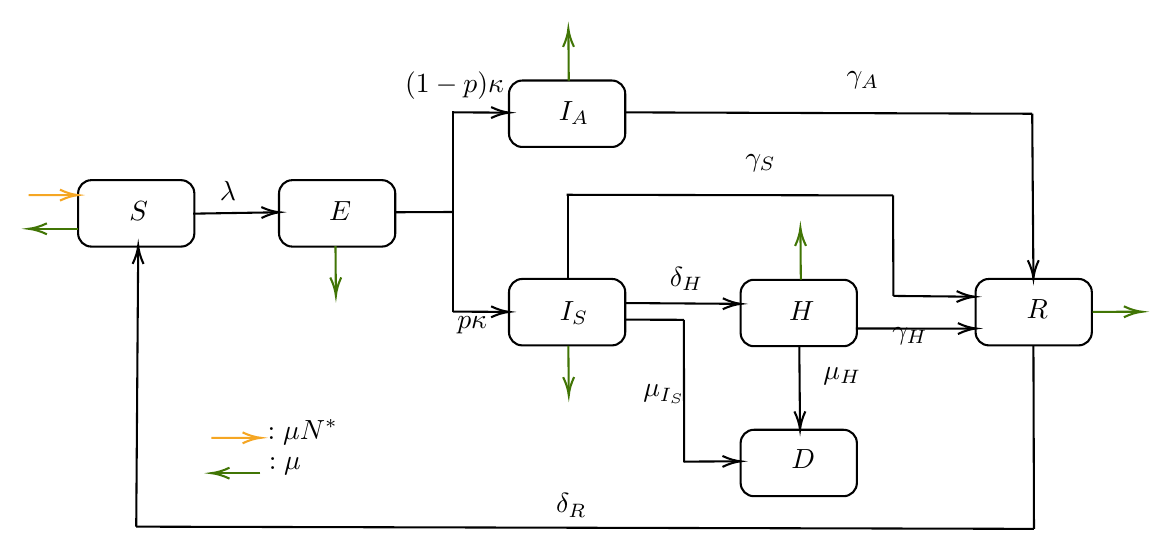
\begin{tikzpicture}[x=0.75pt,y=0.75pt,yscale=-0.8,xscale=0.8]
%uncomment if require: \path (0,391); %set diagram left start at 0, and has height of 391

%Rounded Rect [id:dp9338258576556762] 
\draw   (40,138) .. controls (40,133.58) and (43.58,130) .. (48,130) -- (102,130) .. controls (106.42,130) and (110,133.58) .. (110,138) -- (110,162) .. controls (110,166.42) and (106.42,170) .. (102,170) -- (48,170) .. controls (43.58,170) and (40,166.42) .. (40,162) -- cycle ;
%Rounded Rect [id:dp03550846434827437] 
\draw   (161,138) .. controls (161,133.58) and (164.58,130) .. (169,130) -- (223,130) .. controls (227.42,130) and (231,133.58) .. (231,138) -- (231,162) .. controls (231,166.42) and (227.42,170) .. (223,170) -- (169,170) .. controls (164.58,170) and (161,166.42) .. (161,162) -- cycle ;
%Rounded Rect [id:dp2096597210016533] 
\draw   (299.5,78) .. controls (299.5,73.58) and (303.08,70) .. (307.5,70) -- (361.5,70) .. controls (365.92,70) and (369.5,73.58) .. (369.5,78) -- (369.5,102) .. controls (369.5,106.42) and (365.92,110) .. (361.5,110) -- (307.5,110) .. controls (303.08,110) and (299.5,106.42) .. (299.5,102) -- cycle ;
%Rounded Rect [id:dp4192775592826552] 
\draw   (299.5,197.5) .. controls (299.5,193.08) and (303.08,189.5) .. (307.5,189.5) -- (361.5,189.5) .. controls (365.92,189.5) and (369.5,193.08) .. (369.5,197.5) -- (369.5,221.5) .. controls (369.5,225.92) and (365.92,229.5) .. (361.5,229.5) -- (307.5,229.5) .. controls (303.08,229.5) and (299.5,225.92) .. (299.5,221.5) -- cycle ;
%Rounded Rect [id:dp9412674774350195] 
\draw   (580.5,197.5) .. controls (580.5,193.08) and (584.08,189.5) .. (588.5,189.5) -- (642.5,189.5) .. controls (646.92,189.5) and (650.5,193.08) .. (650.5,197.5) -- (650.5,221.5) .. controls (650.5,225.92) and (646.92,229.5) .. (642.5,229.5) -- (588.5,229.5) .. controls (584.08,229.5) and (580.5,225.92) .. (580.5,221.5) -- cycle ;
%Rounded Rect [id:dp7750331540351684] 
\draw   (439,288.33) .. controls (439,283.92) and (442.58,280.33) .. (447,280.33) -- (501,280.33) .. controls (505.42,280.33) and (509,283.92) .. (509,288.33) -- (509,312.33) .. controls (509,316.75) and (505.42,320.33) .. (501,320.33) -- (447,320.33) .. controls (442.58,320.33) and (439,316.75) .. (439,312.33) -- cycle ;
%Rounded Rect [id:dp22729858034129236] 
\draw   (439,198) .. controls (439,193.58) and (442.58,190) .. (447,190) -- (501,190) .. controls (505.42,190) and (509,193.58) .. (509,198) -- (509,222) .. controls (509,226.42) and (505.42,230) .. (501,230) -- (447,230) .. controls (442.58,230) and (439,226.42) .. (439,222) -- cycle ;
%Straight Lines [id:da8056305543799926] 
\draw    (109.33,150.17) -- (159.33,149.37) ;
\draw [shift={(161.33,149.33)}, rotate = 539.0799999999999] [color={rgb, 255:red, 0; green, 0; blue, 0 }  ][line width=0.75]    (10.93,-3.29) .. controls (6.95,-1.4) and (3.31,-0.3) .. (0,0) .. controls (3.31,0.3) and (6.95,1.4) .. (10.93,3.29)   ;
%Straight Lines [id:da2787683579538649] 
\draw    (230.78,149.33) -- (265.67,149.17) ;
%Straight Lines [id:da21916666537860907] 
\draw    (265.67,89.17) -- (297.67,89.32) ;
\draw [shift={(299.67,89.33)}, rotate = 180.28] [color={rgb, 255:red, 0; green, 0; blue, 0 }  ][line width=0.75]    (10.93,-3.29) .. controls (6.95,-1.4) and (3.31,-0.3) .. (0,0) .. controls (3.31,0.3) and (6.95,1.4) .. (10.93,3.29)   ;
%Straight Lines [id:da8438200798129222] 
\draw    (265.67,88.6) -- (265.67,209.17) ;
%Straight Lines [id:da7337155371803761] 
\draw    (265.67,209.17) -- (297.67,209.32) ;
\draw [shift={(299.67,209.33)}, rotate = 180.28] [color={rgb, 255:red, 0; green, 0; blue, 0 }  ][line width=0.75]    (10.93,-3.29) .. controls (6.95,-1.4) and (3.31,-0.3) .. (0,0) .. controls (3.31,0.3) and (6.95,1.4) .. (10.93,3.29)   ;
%Straight Lines [id:da509274682669141] 
\draw    (369.43,204) -- (424.2,204.39) -- (437.2,204.49) ;
\draw [shift={(439.2,204.5)}, rotate = 180.41] [color={rgb, 255:red, 0; green, 0; blue, 0 }  ][line width=0.75]    (10.93,-3.29) .. controls (6.95,-1.4) and (3.31,-0.3) .. (0,0) .. controls (3.31,0.3) and (6.95,1.4) .. (10.93,3.29)   ;
%Straight Lines [id:da3183759306298827] 
\draw    (405,299.5) -- (437,299.34) ;
\draw [shift={(439,299.33)}, rotate = 539.72] [color={rgb, 255:red, 0; green, 0; blue, 0 }  ][line width=0.75]    (10.93,-3.29) .. controls (6.95,-1.4) and (3.31,-0.3) .. (0,0) .. controls (3.31,0.3) and (6.95,1.4) .. (10.93,3.29)   ;
%Straight Lines [id:da6861028849351065] 
\draw    (370,214) -- (404.8,214.1) ;
%Straight Lines [id:da9190171216881116] 
\draw    (404.8,214.1) -- (405,300) ;
%Straight Lines [id:da03313994658252273] 
\draw    (508.33,219.33) -- (565.2,219.39) -- (578.78,219.34) ;
\draw [shift={(580.78,219.33)}, rotate = 539.78] [color={rgb, 255:red, 0; green, 0; blue, 0 }  ][line width=0.75]    (10.93,-3.29) .. controls (6.95,-1.4) and (3.31,-0.3) .. (0,0) .. controls (3.31,0.3) and (6.95,1.4) .. (10.93,3.29)   ;
%Straight Lines [id:da6934604539767528] 
\draw    (474.33,230) -- (474.76,278.22) ;
\draw [shift={(474.78,280.22)}, rotate = 269.49] [color={rgb, 255:red, 0; green, 0; blue, 0 }  ][line width=0.75]    (10.93,-3.29) .. controls (6.95,-1.4) and (3.31,-0.3) .. (0,0) .. controls (3.31,0.3) and (6.95,1.4) .. (10.93,3.29)   ;
%Straight Lines [id:da6916456040068684] 
\draw    (369,89.17) -- (614.6,90) ;
%Straight Lines [id:da7246498566982733] 
\draw    (614.6,90) -- (615.32,187.17) ;
\draw [shift={(615.33,189.17)}, rotate = 269.58] [color={rgb, 255:red, 0; green, 0; blue, 0 }  ][line width=0.75]    (10.93,-3.29) .. controls (6.95,-1.4) and (3.31,-0.3) .. (0,0) .. controls (3.31,0.3) and (6.95,1.4) .. (10.93,3.29)   ;
%Straight Lines [id:da5396778112959429] 
\draw    (335,139.17) -- (335,189.5) ;
%Straight Lines [id:da7180507787496266] 
\draw    (334.2,138.8) -- (530.8,139.2) ;
%Straight Lines [id:da3365589163505732] 
\draw    (531,199.71) -- (578,200.18) ;
\draw [shift={(580,200.2)}, rotate = 180.57] [color={rgb, 255:red, 0; green, 0; blue, 0 }  ][line width=0.75]    (10.93,-3.29) .. controls (6.95,-1.4) and (3.31,-0.3) .. (0,0) .. controls (3.31,0.3) and (6.95,1.4) .. (10.93,3.29)   ;
%Straight Lines [id:da7818385183529692] 
\draw    (530.8,139.2) -- (531,199.71) ;
%Straight Lines [id:da7484740849372823] 
\draw    (75,338.67) -- (76.19,171.5) ;
\draw [shift={(76.2,169.5)}, rotate = 450.41] [color={rgb, 255:red, 0; green, 0; blue, 0 }  ][line width=0.75]    (10.93,-3.29) .. controls (6.95,-1.4) and (3.31,-0.3) .. (0,0) .. controls (3.31,0.3) and (6.95,1.4) .. (10.93,3.29)   ;
%Straight Lines [id:da29835177923282885] 
\draw    (75,338.67) -- (615.67,340) ;
%Straight Lines [id:da7139155616312535] 
\draw    (615.33,229.67) -- (615.67,340) ;
%Straight Lines [id:da20994732667721105] 
\draw [color={rgb, 255:red, 245; green, 166; blue, 35 }  ,draw opacity=1 ][fill={rgb, 255:red, 65; green, 117; blue, 5 }  ,fill opacity=1 ]   (10.25,139.04) -- (38,139) ;
\draw [shift={(40,139)}, rotate = 539.9200000000001] [color={rgb, 255:red, 245; green, 166; blue, 35 }  ,draw opacity=1 ][line width=0.75]    (10.93,-3.29) .. controls (6.95,-1.4) and (3.31,-0.3) .. (0,0) .. controls (3.31,0.3) and (6.95,1.4) .. (10.93,3.29)   ;
%Straight Lines [id:da9409632697808414] 
\draw [color={rgb, 255:red, 65; green, 117; blue, 5 }  ,draw opacity=1 ]   (39.75,159.29) -- (12.25,159.29) ;
\draw [shift={(10.25,159.29)}, rotate = 360] [color={rgb, 255:red, 65; green, 117; blue, 5 }  ,draw opacity=1 ][line width=0.75]    (10.93,-3.29) .. controls (6.95,-1.4) and (3.31,-0.3) .. (0,0) .. controls (3.31,0.3) and (6.95,1.4) .. (10.93,3.29)   ;
%Straight Lines [id:da671739616587531] 
\draw [color={rgb, 255:red, 65; green, 117; blue, 5 }  ,draw opacity=1 ]   (195,169.79) -- (195.23,197.54) ;
\draw [shift={(195.25,199.54)}, rotate = 269.52] [color={rgb, 255:red, 65; green, 117; blue, 5 }  ,draw opacity=1 ][line width=0.75]    (10.93,-3.29) .. controls (6.95,-1.4) and (3.31,-0.3) .. (0,0) .. controls (3.31,0.3) and (6.95,1.4) .. (10.93,3.29)   ;
%Straight Lines [id:da4612478738976049] 
\draw [color={rgb, 255:red, 65; green, 117; blue, 5 }  ,draw opacity=1 ]   (335.25,229.79) -- (335.48,257.54) ;
\draw [shift={(335.5,259.54)}, rotate = 269.52] [color={rgb, 255:red, 65; green, 117; blue, 5 }  ,draw opacity=1 ][line width=0.75]    (10.93,-3.29) .. controls (6.95,-1.4) and (3.31,-0.3) .. (0,0) .. controls (3.31,0.3) and (6.95,1.4) .. (10.93,3.29)   ;
%Straight Lines [id:da6463966696699537] 
\draw [color={rgb, 255:red, 65; green, 117; blue, 5 }  ,draw opacity=1 ]   (335.5,70.04) -- (335.27,40.79) ;
\draw [shift={(335.25,38.79)}, rotate = 449.54] [color={rgb, 255:red, 65; green, 117; blue, 5 }  ,draw opacity=1 ][line width=0.75]    (10.93,-3.29) .. controls (6.95,-1.4) and (3.31,-0.3) .. (0,0) .. controls (3.31,0.3) and (6.95,1.4) .. (10.93,3.29)   ;
%Straight Lines [id:da5390055225547872] 
\draw [color={rgb, 255:red, 65; green, 117; blue, 5 }  ,draw opacity=1 ]   (475.25,189.92) -- (475.02,160.67) ;
\draw [shift={(475,158.67)}, rotate = 449.54] [color={rgb, 255:red, 65; green, 117; blue, 5 }  ,draw opacity=1 ][line width=0.75]    (10.93,-3.29) .. controls (6.95,-1.4) and (3.31,-0.3) .. (0,0) .. controls (3.31,0.3) and (6.95,1.4) .. (10.93,3.29)   ;
%Straight Lines [id:da5965287355289506] 
\draw [color={rgb, 255:red, 65; green, 117; blue, 5 }  ,draw opacity=1 ]   (651,209.29) -- (678.75,209.25) ;
\draw [shift={(680.75,209.25)}, rotate = 539.9200000000001] [color={rgb, 255:red, 65; green, 117; blue, 5 }  ,draw opacity=1 ][line width=0.75]    (10.93,-3.29) .. controls (6.95,-1.4) and (3.31,-0.3) .. (0,0) .. controls (3.31,0.3) and (6.95,1.4) .. (10.93,3.29)   ;
%Straight Lines [id:da8186275398290976] 
\draw [color={rgb, 255:red, 245; green, 166; blue, 35 }  ,draw opacity=1 ]   (120.25,285.21) -- (148,285.17) ;
\draw [shift={(150,285.17)}, rotate = 539.9200000000001] [color={rgb, 255:red, 245; green, 166; blue, 35 }  ,draw opacity=1 ][line width=0.75]    (10.93,-3.29) .. controls (6.95,-1.4) and (3.31,-0.3) .. (0,0) .. controls (3.31,0.3) and (6.95,1.4) .. (10.93,3.29)   ;
%Straight Lines [id:da2473783506649132] 
\draw [color={rgb, 255:red, 65; green, 117; blue, 5 }  ,draw opacity=1 ]   (149.75,306.46) -- (122.25,306.46) ;
\draw [shift={(120.25,306.46)}, rotate = 360] [color={rgb, 255:red, 65; green, 117; blue, 5 }  ,draw opacity=1 ][line width=0.75]    (10.93,-3.29) .. controls (6.95,-1.4) and (3.31,-0.3) .. (0,0) .. controls (3.31,0.3) and (6.95,1.4) .. (10.93,3.29)   ;

% Text Node
\draw (69,141) node [anchor=north west][inner sep=0.75pt]   [align=left] {$\displaystyle S$};
% Text Node
\draw (189.33,141.33) node [anchor=north west][inner sep=0.75pt]   [align=left] {$\displaystyle E$};
% Text Node
\draw (327.67,81) node [anchor=north west][inner sep=0.75pt]   [align=left] {$\displaystyle I_{A}$};
% Text Node
\draw (328.33,201.33) node [anchor=north west][inner sep=0.75pt]   [align=left] {$\displaystyle I_{S}$};
% Text Node
\draw (466.33,201) node [anchor=north west][inner sep=0.75pt]   [align=left] {$\displaystyle H$};
% Text Node
\draw (609.33,200.33) node [anchor=north west][inner sep=0.75pt]   [align=left] {$\displaystyle R$};
% Text Node
\draw (467.67,290.67) node [anchor=north west][inner sep=0.75pt]   [align=left] {$\displaystyle D$};
% Text Node
\draw (153,295.17) node [anchor=north west][inner sep=0.75pt]   [align=left] {$\displaystyle :\mu $};
% Text Node
\draw (152.33,272) node [anchor=north west][inner sep=0.75pt]   [align=left] {$\displaystyle :\mu N^{*}$};
% Text Node
\draw (123.5,128.67) node [anchor=north west][inner sep=0.75pt]   [align=left] {$\displaystyle \lambda $};
% Text Node
\draw (266.5,210.5) node [anchor=north west][inner sep=0.75pt]   [align=left] {$\displaystyle p\kappa $};
% Text Node
\draw (235,63) node [anchor=north west][inner sep=0.75pt]   [align=left] {$\displaystyle ( 1-p) \kappa $};
% Text Node
\draw (501,63) node [anchor=north west][inner sep=0.75pt]   [align=left] {$\displaystyle \gamma _{A}$};
% Text Node
\draw (440,112.5) node [anchor=north west][inner sep=0.75pt]   [align=left] {$\displaystyle \gamma _{S}$};
% Text Node
\draw (394.5,180.5) node [anchor=north west][inner sep=0.75pt]   [align=left] {$\displaystyle \delta _{H}$};
% Text Node
\draw (487,241) node [anchor=north west][inner sep=0.75pt]   [align=left] {$\displaystyle \mu _{H}$};
% Text Node
\draw (528.5,217) node [anchor=north west][inner sep=0.75pt]   [align=left] {$ $$\displaystyle \gamma _{H}$};
% Text Node
\draw (378.5,251.5) node [anchor=north west][inner sep=0.75pt]   [align=left] {$\displaystyle \mu _{I_{S}}$};
% Text Node
\draw (326,317) node [anchor=north west][inner sep=0.75pt]   [align=left] {$\displaystyle \delta _{R}$};


\end{tikzpicture}

\begin{equation}
    \label{eqn:vacination_dynamics}
    \begin{aligned}
        L' =&  \theta \mu N^{\star}
                -(\epsilon \lambda + \delta_L + \lambda_V +\mu) L
        \\
        S' =&
            (1 - \theta) \mu N^\star
            + \delta_L L
            + \delta_V V
            + \delta_R R
            \\
            &-
            \left(
                \lambda + \lambda_V + \mu
            \right) S
        \\
        E' =&
                \lambda (\epsilon L + (1-\varepsilon) V + S)
                - (\kappa + \mu) E
        \\
        I_S' =&
            p \kappa E
            -
            (
                \delta_H +
                \gamma_S +
                \mu_{I_S} +
                \mu
            ) I_S
        \\
        I_A' = &
                (1 - p) \kappa E - (\gamma_A + \mu) I_A
        \\
        H' = &
            \delta_H I_S - (\gamma_H + \mu_H + \mu) H
        \\
        R' = &
            \gamma_S I_S +
            \gamma_A I_A +
            \gamma_H H
                - (\delta_R + \mu) R
        \\
        D'  = &
                \mu_{I_S} I_S + \mu_H H
        \\
        V' = &
            \lambda_V  (S + L)
            - \left[
                (1 - \varepsilon) \lambda
                + \delta_V
                + \mu
            \right ] V
        \\
        \\
            \frac{dX_{vac}}{dt}
                &=
                (u_V(t) + \lambda_V)
                \left[
                    L + S + E + I_A + R
                \right]
        \\
            \frac{d Y_{I_S}}{dt}
                & = p \kappa E
        \\
            \lambda &:=
                \frac{\beta_A I_A + \beta_S I_S}{N^{\star}}
        \\
        \\
            L(0) &= L_0,
            \ S(0) = S_0,
            \ E(0) = E_0,
        \\
            I_S(0) &= I_{S_{0}},
            I_A(0) = I_{A_{0}},
            H(0) = H_0,
        \\
            R(0) &= R_0, \ D(0) = D_0,
      \\
            V(0) &= 0, \ X_{vac}(0) = 0, \quad
      \\
            X_{vac}(T) &= x_{coverage},
      \\
            N^{\star}(t) &=
                L + S +E + I_S + I_A +
                H + R + V .
        \end{aligned}
\end{equation}
